\documentclass{article}
\usepackage{listings}
\usepackage{graphicx}

\newcommand{\SolutionName}{LeapYear}
\newcommand{\ProjectName}{ZuneDate}

\newcommand{\code}[1]{\lstinline{#1}}

\title{Leap Year Sample}
\date{}


\begin{document}
\maketitle
\begin{abstract}
This sample shows how to use the static checker to do a form of
``abstract debugging'' by examining the termination property of a loop
computing the year and day given the number of days since 1980.  It
also exemplifies how the expressiveness of contracts enables this kind
of debugging across procedure boundaries by means of communicating
established invariants.

\end{abstract}

\newcommand\codefamily\sffamily
\lstset{language={[Sharp]C},mathescape=true,flexiblecolumns=true,morekeywords={Requires,Ensures,Invariant},basicstyle=\codefamily\small,literate={->}{{$\rightarrow$}}{2}{<<}{{$\langle$}}{2}{>>}{{$\rangle$}}{2}{!}{{\textbf{!}}}{2},frame=lines,moredelim=[is][\itshape]{@}{@},captionpos=b,numberstyle=\tiny,stepnumber=1,numbersep=2pt}

\section{Adding the Contract Library Reference}
If you are using Visual Studio 2008, or if you for 
some reason want to target a pre-v4 .NET runtime, then you need to:
\begin{itemize}
\item Change the target framework of the project.
\item Manually add a reference to Microsoft.Contracts.dll
\end{itemize}
Otherwise, you may skip this section and go directly the next section!

To add the reference, open the
\textsf{\SolutionName{}} solution and right-click on
\textsf{References} in the \textsf{\ProjectName{}} project and
select \textsf{Add Reference}. Find the \textsf{Microsoft.Contracts}
library in the \textsf{.NET} tab as shown below and click OK.
\begin{center}
  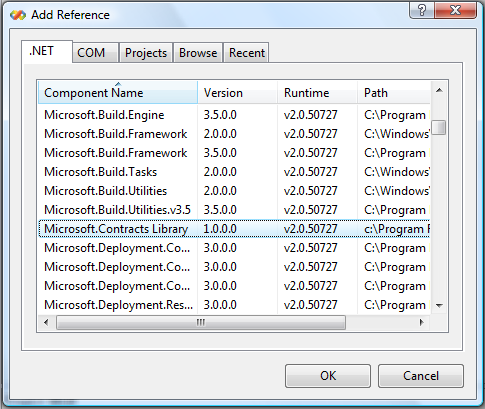
\includegraphics[width=.7\columnwidth]{../Common/addRef.png}
\end{center}



\section{Enabling Static Checking}
\label{sec:start}

After adding the proper reference, go to the Properties of project
\textsf{\ProjectName}, select the Code Contracts pane (at the bottom), and enable static
checking by clicking on the static checking box. 
\begin{center}
  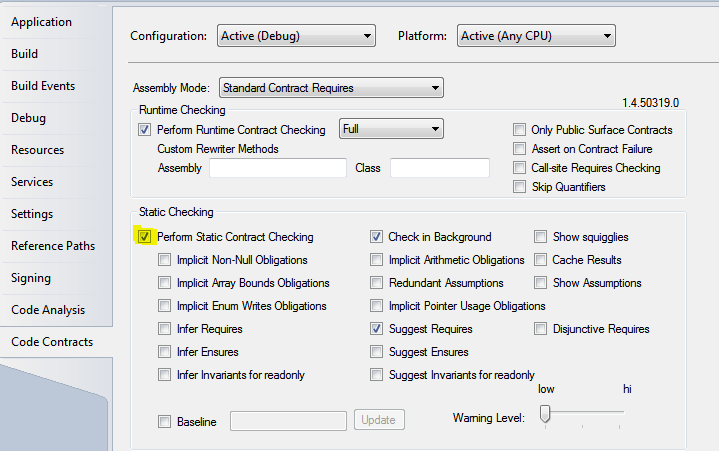
\includegraphics[width=.8\columnwidth]{pane.png}
\end{center}

\section{Overview}
On December 31st, 2008, some older Zune models hung during boot. The
error turned out to be in some BIOS code that computes the current
year from the number of days since 1980. Take a look at the method
\lstinline{YearSince1980} in ZuneDate.cs.

The method's intention is to compute the current year and the day
within that year, given the number of days since 1980. It does so by
repeatedly subtracting 365 days from the days left, until the
remaining days fall within a year. Of course, the code has to take
care of leap years and subtract 366 days in that case.

\section{Proving Termination with Variants}
A variant of a loop is the quantity that decreases on each
iteration. If a loop has a variant and the loop exit
condition triggers when the variant reaches a certain point, then the
loop terminates.

In our example, the loop variant should be the number of days left or
\lstinline{daysLeft}. As we can see, the loop exits when we reach
\lstinline{daysLeft <= 365}. To prove termination, all we have to do
is show that \lstinline{daysLeft} decreases on each iteration.

To do so, let's add the following 2 lines of code around the existing
loop body:
\begin{lstlisting}
      while (daysLeft > 365)
      {
        var oldDaysLeft = daysLeft;
        <existing loop>
        Contract.Assert(daysLeft < oldDaysLeft);
      }
\end{lstlisting}
Remember you can use the code snippet \code{cca TAB TAB} to insert a call to
\code{Contract.Assert}.
Build the project. The build should succeed. After a
moment\footnote{The static checker runs in the background after the regular build.}, 
the static checker should warn that the assert we just added is
unproven (ignore any warnings you might be getting from the Client
project at this point).
\begin{center}
  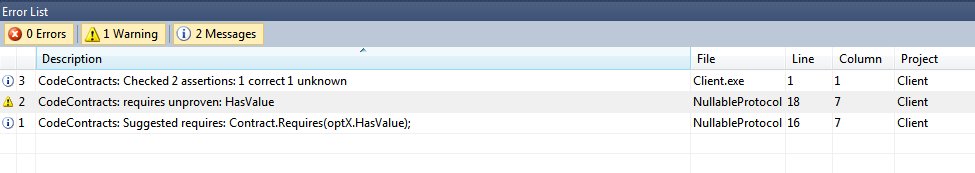
\includegraphics[width=1\columnwidth]{errors1.png}
\end{center}

This tells us that indeed, there might be a problem with the
termination of this loop. If you look more closely at the loop body,
you'll see the inner \lstinline{if} has no \lstinline{else}, which
is suspicous. Let's test our hypothesis that going through that
missing \lstinline{else} is a problem by adding the following \code{else}-branch
there:
\begin{lstlisting}
          if (daysLeft > 366)
          {
            daysLeft -= 366;
            year += 1;
          }
          else
          {
            Contract.Assert(false);
          }
\end{lstlisting}
Putting an \code{Assert(false)} at a particular program point is a way
of saying, I expect to never reach this point. If we build again, we
get the following warning:
\begin{center}
  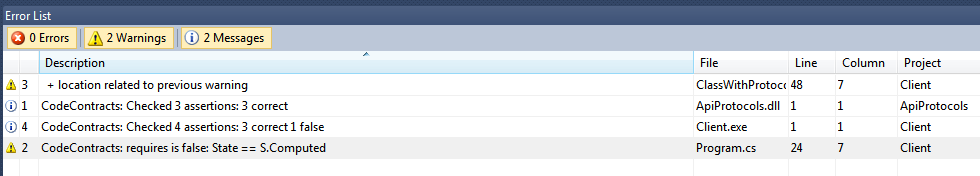
\includegraphics[width=1\columnwidth]{errors2.png}
\end{center}
The \code{Assert(false)} we just added cannot be proven, meaning 
the checker thinks that it is reachable. Note however that the assert
at the end of the loop asserting our variant is now proven. The
checker reasons that since the Assert(false) expresses that we should never get to the
\code{else}-branch, it will only consider all the other control flow
paths. For the remaining paths, it can prove that the loop will
terminate.

\section{Fixing the Code}
Let's examine what should happen in the problematic
\code{else}-branch. We get into the else branch when we have more
than 365 days left, the year is a leap year, but there are not more
than 366 days left. Well, this means that
\code{daysLeft} is exactly 366. Let's test this insight with an
assertion:
\begin{lstlisting}
          else
          {
            Contract.Assert(daysLeft == 366);
            Contract.Assert(false);
          }
\end{lstlisting}
Build and look at the warnings. You'll see that it proves this assert
correct, as it still complains about the \code{Assert(false)}. Good,
our intuition is correct. Now what should happen in this case? We are
in a leap year and we have 366 days left. This means we are on the
last day of this leap year, namely December 31st. In this case, the
method should return the year and the day in the year should be 366.

Let's fix the code by changing the \code{else}-branch to the
following:
\begin{lstlisting}
          else
          {
            dayInYear = daysLeft;
            return year;
          }
\end{lstlisting}
We could of course just set \code{dayInYear} to 366, as we have just
shown that it will be the case.
Now let's rebuild and see what the checker tells us.
\begin{center}
  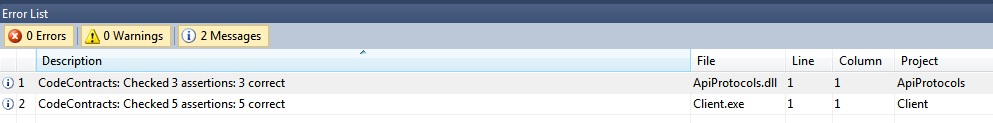
\includegraphics[width=1\columnwidth]{errors3.png}
\end{center}
Now the checker proves the assert at the end of the loop that the
\code{daysLeft} decreases each time around the loop. Thus we can be
assured that the loop
terminates. 

So far, we have used the static checker to perform ``abstract
debugging'' without ever running the code. By seeing which program
points are reachable and verifying our hypotheses by inserting
assertions that the checker then tries to discharge, we discovered the
missing corner case and validated our assumption that it happens when
the day is the last day of a leap year.

For this simple example, we didn't need any further contracts. In the
next sections, we show how contracts can help provide this kind of
abstract debugging for callers of code.

\section{Checking the Client}

Now it is time to look at the client in Program.cs. Let's enable
static checking on the \code{Client} project, including array bound
validation:
\begin{center}
  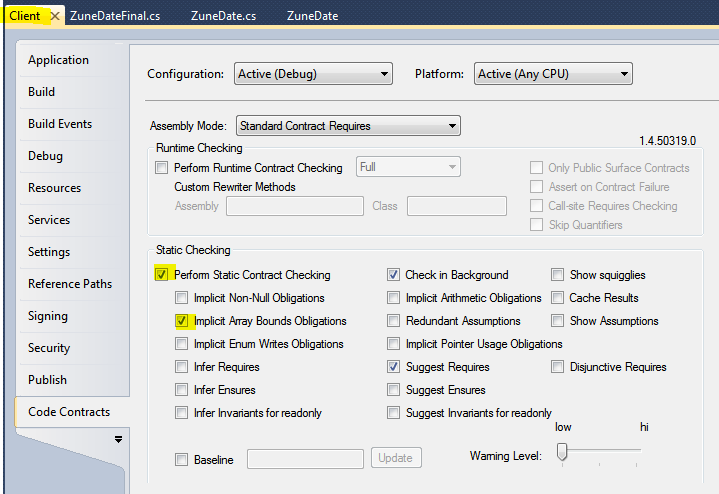
\includegraphics[width=1\columnwidth]{pane2.png}
\end{center}
Build the \code{Client} project (or the solution). The checker will
report that it cannot prove the array access below:
\begin{lstlisting}
      days[dayInYear] = "used";
\end{lstlisting}
The client code seems to be getting a day since 1980 from the command
line, calling \code{YearSince1980}, allocating an array of days of
size 366, and then assigning to the element specified by the returned
\code{dayInYear}.

Why is the static checker not able to prove the array access as safe?
After all, we just looked through the \code{YearSince1980} method and
saw that it returns the day in the year.

We can try to narrow down the problem by inserting assertions about
these assumptions right after the method call to \code{YearSince1980}.
\begin{lstlisting}
      int year = ZuneDate.YearSince1980(daysSince1980, out dayInYear);
      Contract.Assert(dayInYear >= 0);
      Contract.Assert(dayInYear <= 366);
\end{lstlisting}
Let's run the checker again and see what it thinks.
\begin{center}
  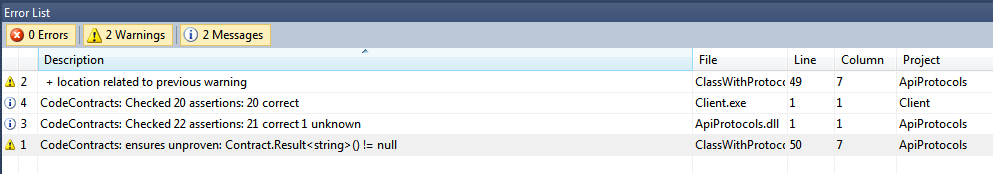
\includegraphics[width=1\columnwidth]{errors4.png}
\end{center}
The checker cannot prove either of our assertions. But note that it
now complains only about the upper bound of the array. Thus, if the
\code{Assert(dayInYear >=0)} is true, the array bound access later is
at least respecting the lower bound of the array. Why isn't it also
proving the upper bound?

The answer is of course that arrays are 0 indexed, but days in the
year are between 1..366. Our array has valid indices between 0..365.
This is a classical ``off-by-one'' error. Let's correct it:
\begin{lstlisting}
      days[dayInYear - 1] = "used";
\end{lstlisting}
and rebuild the project.
\begin{center}
  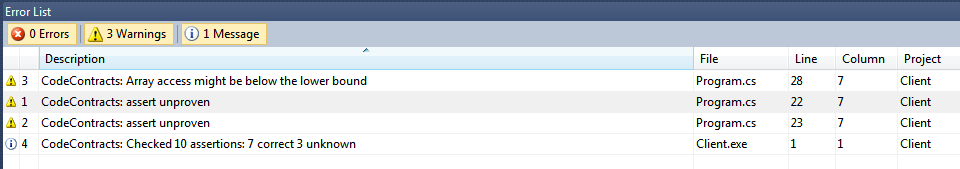
\includegraphics[width=1\columnwidth]{errors5.png}
\end{center}
Look at the third warning about the array access: now the checker is
complainng that the lower bound may not be respected, but the upper
bound is now okay. Looking back at our assertions, we can see that we
only asserted \code{dayInYear >= 0}, where as the code later assumes
\code{dayInYear >= 1}. Let's fix the assert.
\begin{lstlisting}
      Contract.Assert(dayInYear >= 1);
\end{lstlisting}
and rebuild. Now the checker should only warn about the two assertions,
but no longer about the array accesses, since the assertions are now
enough to imply that the array access will be within bounds.

How can we prove these asserts correct now? The static checker works
modularly, one method at a time, using the contracts of called methods
to understand what is going on at method call sites. In this case,
there are no contracts on \code{YearSince1980}, and thus the static
checker will assume that \code{dayInYear} in the \code{Main} method
could be any integer. That's why the assertions are not proven. To fix
this, we need to go back to \code{YearSince1980} and add
contracts there.

\section{Contracts on YearSince1980}

The assumption the client is making about the return value of
\code{dayInYear} is that it is between 1 and 366. Let's make this
explicit as a post condition of the method:
\begin{lstlisting}
    public static int YearSince1980(int daysSince1980, out int dayInYear)
    {
      Contract.Ensures(Contract.ValueAtReturn(out dayInYear) >= 1);
      Contract.Ensures(Contract.ValueAtReturn(out dayInYear) <= 366);
\end{lstlisting}
Note how we need to use the method \code{Contract.ValueAtReturn} to
refer to the final value of out-parameters of a method.
Currently the tools do not check to make sure that out
parameters are initialized properly disregarding their mention in the
postcondition. Thus, in the above example, if the code after the
contracts uses the value of \code{dayInYear} before assigning to it, the C\#
compiler would not issue the error that it should. However, on a build
where the \code{CONTRACTS_FULL} is not defined (such as
\code{Release}), the compiler will issue an error.

Build the
\code{ZuneDate} project and observe the output:
\begin{center}
  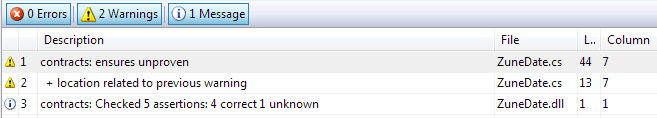
\includegraphics[width=1\columnwidth]{errors6.png}
\end{center}
The checker validates the upper bound (366) on the final value of
\code{dayInYear}, but not the lower bound of 1. If you consider the
code for a second, you will notice that indeed a negative parameter
would cause that problem, as the loop would then never execute.

To avoid this, let's add the necessary pre-condition:
\begin{lstlisting}
    public static int YearSince1980(int daysSince1980, out int dayInYear)
    {
      Contract.Requires(daysSince1980 >= 1);
\end{lstlisting}
Now rebuild the entire solution. You should see that the checker
validates all contracts on the \code{ZuneDate} project, but that there
is now a violated requires in the client.
\begin{center}
  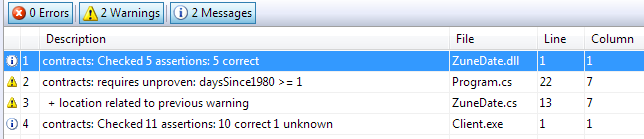
\includegraphics[width=1\columnwidth]{errors7.png}
\end{center}
The client code does not perform any validation on the parsed
\code{daysSince1980} value before passing it to \code{YearsSince1980},
thus, the value may not be positive.  We can easily fix the client
code by writing the extra return below before computing the year:
\begin{lstlisting}
      int daysSince1980 = Int32.Parse(args[0]);
      if (daysSince1980 <= 0) return;
\end{lstlisting}
When you rebuild, the checker should now validate the client code as
well.

\section{More Detailed Contracts}
Now suppose the client code programmer were really worried about
memory consumption and wants to allocate an array that matches the
number of days needed exactly, rather than overprovisioning for leap
years. In other words, the client code in \code{Main} changes as follows:
\begin{lstlisting}
      int dayInYear;
      int year = ZuneDate.YearSince1980(daysSince1980, out dayInYear);

      string[] days;
      if (DateTime.IsLeapYear(year))
      {
        days = new string[366];
      }
      else
      {
        days = new string[365];
      }
      days[dayInYear - 1] = "used";
\end{lstlisting}
As you can see, we now allocate either 366 or 365 elements for the
\code{days} array, depending on the leap year status of the returned
year. When you build, the checker will report that it no longer proves
the upper bound on the array access. 

The reason for this warning is the same as at the beginning of this
sample. The contract on method \code{YearSince1980} is not detailed
enough to specify that in case the returned year is not a leap year,
then the \code{dayInYear} is bounded by 365.

Fortunately, if we want to, we can actually specify this and also
check that the implementation satisfies this property. Going back to
the implementation of \code{YearSince1980}, add the following
postcondition:
\begin{lstlisting}
  Contract.Ensures(DateTime.IsLeapYear(Contract.Result<int>())
                   || Contract.ValueAtReturn(out dayInYear) <= 365);
\end{lstlisting}
The specification states that either the returned year is a leap year,
or the final \code{dayInYear} value is bounded by 365. When you
rebuild the solution, you should see that the new postcondition is
proven, meaning our date computation is looking pretty solid.


\end{document}
